
一般来说,我们需要修改的现有代码越少,设计的可改动性就越大:
需要修改的代码越少,意味着需要做的工作就越少(效率),犯错误的可能性就越小(有效性)。
我们需要处理的地方更少(切换-效率),犯错误的机会更少(有效性)。

\paragraph{可变性应当是固定的}如果设计没有改变,其可变性也不应当改变。这意味着可变性应该与我们想要实施的具体更改无关。换句话说,无论我们要进行的更改有多大,现有设计的可变性应该是相同的。例如,无论是为井字游戏添加图形用户界面还是仅仅将`X'改为`x'和`0'改为`o',现有设计的可变性都应该相同。

\paragraph{可变性与新增代码的数量无关}实际上,这意味着可变性不应依赖于必须编写的新代码数量。但是,什么是新代码?

在现有代码行中添加代码? — 这是对现有代码行的更改。

在现有方法中添加完整的代码行? — 这是对现有方法的更改。

添加新方法? — 这是对现有类的更改。

添加新的内嵌类? — 这是对现有类的更改。

添加枚举? — 如果是内嵌的,则是对现有类的更改。

添加枚举? — 如果是新文件,则是新的。

新接口? — 如果是新文件,则是新的。

新类? — 如果是新文件,则是新的。

\paragraph{评估可变性时应忽略新文件}换句话说,当考虑设计的可变性时,我们应该关注对现有设计元素的更改,而不是完全新的添加。如果在添加新功能的时候完全没有改动旧代码,那就太好了。

\section*{量化可更改性}
\subsubsection{CR值}
CR 通过比较预期的变更影响(I)和实际必须更改的类或文件的数量来评估可变性。理想情况下,如果一个系统是高度可维护的,对于一个给定的变更,需要更改的文件数量应该是最小化的。
\[\displaystyle CR = \frac{C}{N}\]
其中,N 是现有设计中的类(或文件)总数。
C 是实现变更案例时需要更改的类(或文件)数量。

如果 $CR \approx I$,变更成本与预期一致。
如果 $CR > I$,则变更成本高于预期,表明系统的可变性较低(即更难修改)。
如果 $CR < I$,则变更成本低于预期,表明系统的可变性较高(即更易修改)。

\subsubsection{降低CR值--增加N}
千方百计添加类来增加N(look for excuses to add classes!)。这可能涉及对系统进行更细粒度的分解,每个类都有一个非常特定的责任。

\subsubsection{降低CR值--减少C}
强调尽可能在新的类中添加新代码,而不是更改现有的类。这种策略有助于保持现有代码的稳定性,同时允许扩展和修改。

\subsubsection{局限性}
CR是一个针对特定变更案例的度量标准,它不能全面地代表一个设计的整体可变性。一个设计在某一特定变更案例下可能表现出低CR(即高可变性),但在另一个变更案例下可能就表现出高CR(即低可变性)。

实际的变更案例是无限的,所以我们无法确保已经考虑了所有可能的变更案例。这在某种程度上限制了CR度量的全面性和预测性。

当系统规模庞大(例如,类的数量以千计)时,未实际进行变更之前,很难准确地确定需要变更的类的数量(C),这进一步增加了使用CR的复杂性。

模型是相当粗粒度(coarse-grained)的,因为它不考虑更改的方法或语句。这意味着,即使更改影响到了多个类,如果每个类只需要很小的更改,CR 也可能高估了实际变更成本。

考虑到这些局限性,建议在做设计决策时,寻找能够在可能发生的、具有实质性影响的变更案例下最小化CR的设计。应该避免那些CR高度依赖于特定变更案例的设计,因为这种设计的可变性更难以预测和管理。寻找能减少需要变更的类的数量的设计,或者在保持需要变更的类数量不变的情况下增加总类数量的设计。这可能涉及到更细粒度的模块化,或者更好的封装和抽象。
对任何设计,都应该思考可能引起问题的变更案例,并尝试预测和规划这些情况。这样的前瞻性思考可以帮助创建一个更具弹性和适应性的系统设计。

\chapter{Design Patterns}

\section{好的设计}
设计模式最初是由 Gamma, Helm, Johnson, Vlissides 提出,他们也被称为“四人帮”(Gang of Four, GoF)。设计模式是从多年的对象导向设计经验中提炼出的精华,它提供了一种框架,让开发者能够解决反复出现的设计问题,而不必每次都从头开始。

设计模式不是针对特定问题的具体实现,而是\textbf{对在特定上下文中反复出现的问题的通用解决方案。}因此,它们提供了一种方法,帮助开发者识别问题,并应用已经验证过的解决方案,这有助于提高开发效率并减少错误。

设计模式描述的是一种通用解决方案,而不是一种特定的实现。这意味着,虽然设计模式提供了结构和方法论,但它们可以根据具体需求进行调整和修改。这种灵活性允许设计模式在不同的情况下以不同的方式实现。

设计模式的有效性取决于它们被应用的上下文。如果上下文发生变化,可能原本适用的设计模式就不再适用。因此,理解和识别正确的上下文是应用设计模式的关键。

尽管设计模式本身\textbf{并不直接支持可变性(Alterability)},但许多设计模式都是为了解决与变化支持有关的问题而创建的。因此,它们往往间接地影响了系统的可变性,使得软件能够更容易适应变化,从而提高了其长期的可维护性和灵活性。


\paragraph{使用了设计模式的设计就一定是好的设计吗?}设计模式的使用量与设计质量不成正比,要考虑到设计模式的适用性和上下文相关性。

设计模式是为特定上下文中的特定问题而创建的。如果一个设计模式解决的问题与当前需要解决的问题不匹配,或者设计模式预期的上下文与实际应用的上下文不一致,那么使用该设计模式不能被认为是“好的设计”。在这种情况下,即使是经过验证的设计模式也可能导致不必要的复杂性、性能下降或其他问题。

\section{Composite 复合模式}

复合模式的主要目的是允许客户端统一对待单个对象和对象的组合。这种模式主要用于希望以相同方式对待个别对象和组成对象的复杂结构,尤其是在具有部分-整体层次结构的情况下。通过这种方式,客户端不需要区分它们在处理的是单个对象还是对象的集合。这种模式解决的核心问题是如何有效地表示部分-整体层次结构。在这样的结构中,组件既可以是单个对象(部分)也可以是包含多个对象的组(整体)。复合模式适用于希望统一处理单个元素和元素集合的情况。这在各种应用中都很常见,例如图形系统(其中对象可以是单个形状或形状的组合)、文件系统(其中对象可以是文件或文件夹)等。

\begin{figure}[h]
    \centering
    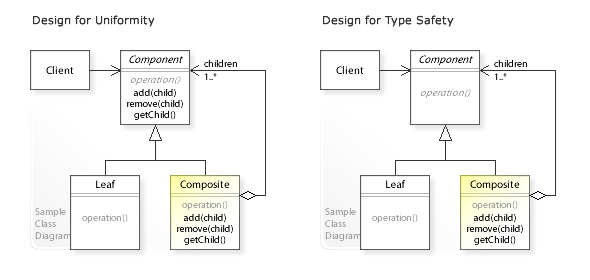
\includegraphics[width=8cm]{res/W3sDesign_Composite_Design_Pattern_Type_Safety_UML.jpg}
    \caption{Composite Pattern}
\end{figure}


这种模式通常包括三个主要元素:
\begin{itemize}
	\item 组件(Component) - 是一个抽象类或接口,定义了叶子和复合对象的公共接口。客户端通过这个接口与所有对象交互,无需关心它们是单个对象还是组合。
	\item 叶子(Leaf) - 表示单个对象,实现或继承自组件接口。它没有子元素。
	\item 复合(Composite) - 表示对象的集合,也实现或继承自组件接口。它内部包含组件列表,并可能提供添加、删除或获取组件的方法。
	
\end{itemize}

\subsubsection{基本流程}

\begin{itemize}
	\item 客户端使用Component接口与组合结构中的对象进行交互。如果接收者是一个叶子,那么请求直接处理。如果接收者是一个Composite,它通常将请求转发给它的子部件,在转发前后可能进行一些预处理或后处理。
	\item 在大多数情况下,客户端并不知道正在与之交互的是叶子还是复合组件,它只是针对Component接口进行操作。
\end{itemize}

\subsection{复合模式举例}

\subsubsection{文件系统}
在文件系统中,目录(Directories)和文件(Files)的关系是一个典型的复合模式实例。

目录(Directories, Composite):可以看作复合对象,因为它们可以包含其他目录或文件。目录具有添加、删除或获取其内部内容的功能。

文件(Files, Leaves):可以看作叶子对象,因为它们是文件系统中的终端对象,不包含其他目录或文件。

\begin{lstlisting}[language=Java, caption=Composite Design Pattern Example, label=lst:composite_pattern]
public interface File {
    String longDetails();
    String shortDetails();
}

public class PlainFile implements File {
    private String _name;

    public PlainFile(String name) { ... }

    public String longDetails() {
        return _name;
    }

    public String shortDetails() { ... }
}

public class Directory implements File {
    ...
    private List<File> _contents;

    public Directory(String name, String permissions) {
        ...
        _contents = new ArrayList<File>();
    }

    public void addFile(File file) {
        _contents.add(file);
    }

    public String longDetails() {
        String result = _name + "/ (" + _permissions + ")";
        for (File file: _contents) {
            result += "\n" + file.longDetails();
        }
        return result;
    }

    public String shortDetails() { ... }
}

public class Browser {
    public static void main(String[] args) {
        Directory root = new Directory("root", "drwx------");
        root.addFile(new PlainFile("README"));
        Directory home = new Directory("home", "drwx------");
        root.addFile(home);
        Directory user = new Directory("ewan", "drwxrwxrwx");
        home.addFile(user);
        PlainFile compsci701quiz2 = new PlainFile("MostSecret.tex");
        user.addFile(compsci701quiz2);

        System.out.println("Printing root directory");
        print(root);
        System.out.println("\nPrinting user directory");
        print(user);
        System.out.println("\nPrinting plain file");
        print(compsci701quiz2);
    }

    private static void print(File start) {
        System.out.println(start.longDetails());
    }
}
\end{lstlisting}

在本代码中,复合模式的角色和具体的类对应如下:
\begin{itemize}
	\item Component: File
	\item Composit: Directory
	\item Leaf: PlainFile
	\item Client: Browser
\end{itemize}

\subsubsection{员工层级}
企业中的员工层级结构也是复合模式的一个实例。

部门(Departments, Composite):可以包含其他子部门或单独的员工。部门可以有添加、删除或获取其成员的功能。

个人员工(Individual Employees, Leaves):作为层级结构中的终端对象,不包含其他员工或子部门。

\subsubsection{用户界面框架(如Swing)}

用户界面框架中的组件和容器关系通常遵循复合模式。

容器(如JPanel, Composite):可以包含其他容器或界面组件。它们具有添加、删除或获取其内部组件的功能。

组件(如JButton, Leaves):作为界面中的终端对象,它们是单独的元素,不包含其他组件。

\subsubsection{算术表达式}

算术表达式的构建也可以使用复合模式。

使用运算符的表达式(如加、减、乘、除, Composite):这些表达式可能会包含其他子表达式或值/变量。例如,一个复合表达式可能是3 + (4 * 5),其中4 * 5也是一个复合表达式。

值或变量(如数字、字符, Leaves):作为表达式中的终端对象,它们是单独的元素。

\subsection{评价复合模式}

使用复合模式可以使代码更加简洁和高效。没有复合模式,达到同样的功能将需要更多的代码,并且这些代码会更复杂。

对于熟悉复合设计模式的人,他们会发现这种模式更容易理解,因为它已经在他们的知识库中。
但对于不熟悉该模式的人,可能会感到困惑或难以理解。

\subsubsection{可变性和复合模式}
要添加新的叶子类L:
L是新的代码,所以在评估可变性时,它“不算数”。
至少需要修改一个类来从L构造对象。如果需要修改多于一个的类,那么这可能意味着复合模式并没有按预期的方式实现。
因此,$C\text{(改变的类数)}= 1$。但实际情况可能会有所不同。
添加新的复合类与此相同。
通常,客户端(调用代码)不需要改变。
但要注意的是,如果更改组件,可能需要更改复合类和每一个叶子类。

\section{Command 命令模式}

命令模式的主要目的是将一个请求封装为一个对象,这使得可以为客户端提供不同的请求、将请求排队或记录、并支持可撤销的操作。简而言之,这种模式允许我们将操作(命令)与请求该操作的对象(调用者)和知道如何执行操作的对象(接收者)进行分离。

\begin{figure}[h]
    \centering
    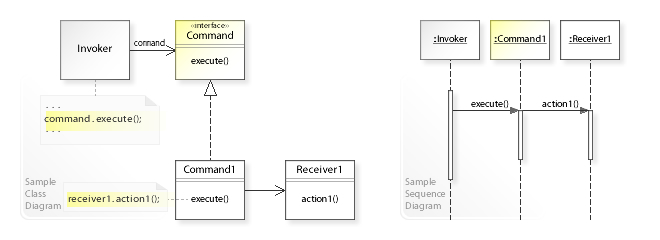
\includegraphics[width=8cm]{res/W3sDesign_Command_Design_Pattern_UML.jpg}
    \caption{Command Pattern}
\end{figure}

核心问题是如何将一个操作的调用者与执行该操作的实体进行解耦。为什么这很重要?因为直接的耦合可能导致代码更难维护、扩展和重构。
解耦的关键是要确保在时间和空间上都进行。这意味着命令可以在不同的时间点被创建、排队、执行或记录,而与命令的执行者和接收者在物理上或逻辑上都没有直接的联系。

命令模式的结构通常包含以下四个主要元素:
\begin{itemize}
	\item 客户端 (Client): 这是初始化命令需求的实体。它知道具体的命令和其参数,并将命令对象传递给调用者。
	\item 命令 (Command): 这是一个抽象的接口或类,定义了执行操作的方法。它通常具有一个execute()方法,该方法调用接收者来执行请求的操作。
	\item 调用者 (Invoker): 它持有命令对象,并在某个点上调用命令对象的execute()方法来执行请求。它不知道命令的具体实现或接收者是什么。
	\item 接收者 (Receiver): 这是命令实际执行操作的实体。它知道如何执行与命令相关的操作。
\end{itemize}

\subsubsection{工作流程}
\begin{itemize}
	\item 客户端创建一个命令对象,并设定它的接收者。
	\item 调用者接收到命令对象,并在某个时间点调用命令对象的execute()方法。
	\item 命令对象向接收者发送请求。
\end{itemize}
\subsection{命令模式应用举例}

\begin{itemize}
	\item 图形用户界面(GUI)操作实现(一般来说,将图形用户界面(GUI)操作与图形用户界面(GUI)本身分离开来)
	\item 延迟执行命令
	\item 记录执行的命令
	\item 更改执行命令的位置
\end{itemize}


\subsection{评价命令模式}
\subsubsection{可变性和命令模式}
当我们希望在已有的系统中添加新的行为或操作时,命令模式为此提供了一种优雅的方法。

\paragraph{添加具体的命令类 (Add concrete command classes)}当需要引入新的行为或操作时,我们可以简单地添加一个新的具体命令类。这是全新的代码,因此从可变性的角度来看,它并不被计入修改的成本中。这意味着我们可以轻松地扩展系统功能,而无需对现有的命令类进行大量修改。

\paragraph{创建具体的命令对象 (Create concrete command objects)}为了在系统中使用新的具体命令类,我们需要在某个地方创建其对象。这可能需要修改现有的代码,特别是在命令对象的创建和管理的地方。根据提供的信息,这应该只修改一个类,即负责创建和管理命令对象的那个类。

\paragraph{可能需要修改选择命令对象的类 (Possibly one other class needs to change to choose the concrete command object to be created)}
除了上述的类,可能还有另一个类需要进行修改,以便选择并创建正确的具体命令对象。这通常是调用者或与命令相关的某个客户端。

\paragraph{典型的改动成本 (Typically $C = 2$)}当引入新的行为时,通常需要修改两个现有的类。这意味着,使用命令模式,系统的可变性通常是可接受的,因为大部分的新增行为只涉及添加新的代码,而对现有代码的修改是有限的。

命令模式提供了一种将操作封装为对象的方法,从而允许系统在不影响其核心结构的前提下进行扩展。在考虑可变性时,它确保了系统的扩展和维护变得更加直接和简单。

\section{Observer 观察者模式}

\subsubsection{目的}
观察者模式的主要目的是定义对象之间的一对多的依赖关系,当一个对象(被观察者)的状态发生变化时,所有依赖它的对象(观察者)都会被自动通知和更新。这种模式常用于实现事件驱动的系统,其中某些对象的状态变化可能会影响到其他对象的行为。

\subsubsection{解耦}
被观察者(或称为“主题”)不应该知道关于观察者的任何信息。这确保了被观察者与观察者之间的解耦,使得在运行时可以轻松地添加或移除观察者。这种解耦是观察者模式的关键特性,因为它允许系统在不修改被观察者代码的前提下增加新的响应行为。

\subsubsection{观察者与被观察者 (Observers and Observed)}

\paragraph{观察者 (Observers)}是对被观察者的状态变化感兴趣的对象。当被观察者的状态发生变化时,观察者希望知道这一变化,以便根据自己的需求做出相应的反应。

观察者需要某种方式来告诉被观察者它们对其状态变化感兴趣。这通常通过注册机制实现,观察者可以注册自己,以便在被观察者状态发生变化时接收通知。

\paragraph{被观察者 (Subject)}是观察者关心的对象,当其状态发生变化时,它会自动通知所有注册的观察者。

当被观察者的状态发生变化时,它可以选择在通知中包含关于变化的具体信息,也可以不包含。这意味着通知可以是通用的(例如“状态已更改”),也可以是具体的(例如“温度已从20°C上升到25°C”)。

\subsubsection{工作流程}

\begin{figure}[h]
    \centering
    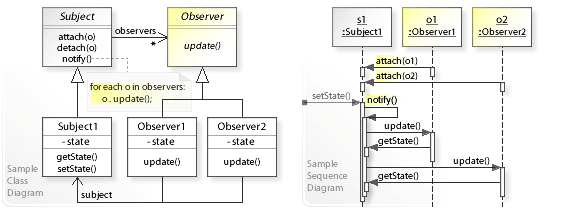
\includegraphics[width=8cm]{res/observer_pattern.png}
    \caption{Observer Pattern}
\end{figure}

\begin{itemize}
	\item 具体主题内部状态发生改变。
	\item 具体主题通知观察者对象,通常通过调用观察者的更新方法。
	\item 每个观察者使用主题的getter方法来同步自己的状态与主题的状态。
\end{itemize}

\subsection{观察者模式应用举例}
记录系统中相关事件并提供这些事件(如写入文件)的日志系统。日志记录器是观察者,它以观察者身份向其希望记录事件的各个组件注册。例如,身份验证组件管理任何试图进行身份验证的用户。每次尝试都会通知日志记录器

\subsection{评价观察者模式}

观察者模式提供了一种强大的方式来实现对象之间的低耦合交互。当一个对象的状态发生变化时,所有对该变化感兴趣的对象都会得到通知,而不需要被观察者知道这些观察者的具体细节。这种模式在很多现代软件设计中都有应用,特别是在事件驱动的应用程序和实时系统中。

\section{Decorator 装饰器模式}

装饰器模式的主要意图是动态地为对象附加额外的职责。与继承相比,装饰器为扩展功能提供了更加灵活的替代方案。当你有一个对象和多个可以独立添加或删除的职责时,使用继承会导致子类数量呈指数级增长。
例如,如果有4种可能的职责,并且任何一种或多种职责都可以附加到一个对象上,那么使用继承可能需要16种子类来覆盖所有可能的组合。
装饰器模式提供了一种避免此问题的解决方案。通过动态地添加装饰器来扩展对象的功能,而不是通过继承创建大量的子类。

一个被装饰的具体组件是一个组件,由其行为被装饰器修改的具体组件组成。

\subsubsection{角色}

\textbf{抽象组件(Component):}
这是一个接口或抽象类,定义了对象的核心接口或核心方法,可以给这些对象动态地添加职责(功能)。

\textbf{具体组件(ConcreteComponent):}
这个角色实现(或继承)了抽象组件,它代表了需要被装饰的原始对象,即可以有附加职责的对象。

\textbf{抽象装饰者(Decorator):}
也是一个接口或抽象类,继承或实现了抽象组件。装饰器类的主要任务是为了增加新功能。
它通常持有一个指向抽象组件的引用,并定义了一个与抽象组件接口一致的接口。

\textbf{具体装饰者(ConcreteDecorator):}
这是实现抽象装饰者的类。它负责增加新的职责,可以扩展一个类的行为或状态。

\subsubsection{工作流程}
\begin{figure}[h]
    \centering
    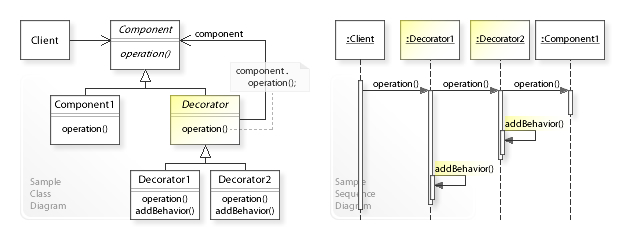
\includegraphics[width=8cm]{res/W3sDesign_Decorator_Design_Pattern_UML.jpg}
    \caption{Decorator Pattern}
\end{figure}

\begin{itemize}
	\item 客户端创建具体组件对象(ConcreteComponent)。
	\item 客户端选择具体装饰者(ConcreteDecorator)并将步骤1中创建的对象传递给它,这可以通过构造方法或者某些设置方法实现。
	\item 客户端如果需要添加额外的职责(功能),则继续用其他具体装饰者包装当前对象。
	\item 客户端调用最终对象的方法进行操作。
\end{itemize}

\subsection{装饰器模式应用举例}

\paragraph{Java 中的Reader层次结构}
例如,BufferedReader 修改了阅读器的行为,增加了缓冲功能。
(实际上,BufferedReader 确实增加了一些行为,而这在技术上是不应该通过 Decorator 来实现的)。

\subsection{评价装饰器模式}

当需要为对象动态地添加职责,而不想使用大量子类时,装饰器模式是理想的选择。
例如,在图形用户界面中,一个窗口可能有多种可能的装饰(如滚动条、边框、标题栏等)。使用装饰器模式可以允许用户在运行时选择哪些装饰应用于窗口,而不是为每种可能的组合创建一个子类。


\section{Factory Method 工厂方法模式}

工厂模式主要关注于对象的创建,属于创建型设计模式。但是它将实际创建对象的任务交给子类来完成。这种分离使得代码更加模块化和可扩展。属于创建型设计模式。

工厂方法模式的核心是定义一个用于创建对象的接口,但是具体决定实例化哪一个类的责任是交给子类的。这意味着基类可以定义创建对象的过程(即工厂方法),但具体的实现细节(创建哪一种产品)是由子类决定的。

很多时候,我们构建框架时会依赖抽象性。这种抽象性让框架更具有通用性和灵活性,因为它不与具体的实现细节绑定。然而,最终这些抽象必须在某处被具体化,因为在实际应用中,我们需要创建具体的对象实例。
工厂方法模式提供了一个答案:如何在保持分离的同时,控制何时和如何创建具体的实例。基类中只定义了如何创建产品的框架(即工厂方法),而具体的产品类型则由子类决定。

在工厂方法模式中,有两个主要组件:产品和工厂。产品是要创建的对象,而工厂是负责创建这些对象的实体。
每个具体的工厂都负责创建一个具体的产品。这种关系很重要,因为它确保了创建对象的过程与实际创建的对象类型之间的一致性和对应关系。

\subsubsection{角色}
\textbf{抽象工厂(Creator)类/接口:}声明工厂方法,该方法返回一个产品类型的对象。

\textbf{具体工厂(Concrete Creator)类:}实现工厂方法,重定义它以返回一个具体产品实例。

\textbf{抽象产品(Product)类/接口:}定义产品的接口,描述产品的主要特性和功能。

\textbf{具体产品(Concrete Product)类:}具体工厂类所创建的对象,实现抽象产品接口。

\subsubsection{工作流程}

\begin{figure}[h]
    \centering
    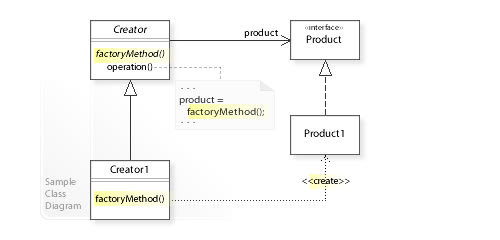
\includegraphics[width=8cm]{res/Factory-Method-UML.jpg}
    \caption{Factory Method Pattern}
\end{figure}
\begin{itemize}
	\item 定义产品接口:首先,会有一个产品接口或抽象类,定义具体产品的通用接口或者实现。这个接口通常包含了产品对象的行为方法。
	\item 具体产品实现:对于每一种具体产品,都有与之对应的具体类实现产品接口或继承自产品抽象类,实现具体的产品对象,并实现产品接口中定义的方法。
	\item 定义工厂接口:这是工厂方法模式的核心。一个工厂接口主要声明一个方法(也叫工厂方法),这个方法返回一个产品接口对象。
	\item 具体工厂实现:对于每个要创建的具体产品,都有一个具体的工厂类与之对应,这个工厂类实现了工厂接口,实现其中的工厂方法,即创建一个具体的产品对象并返回。
	\item 客户端决定:客户端首先选择一个具体的工厂实现并创建之。然后,调用这个工厂对象的工厂方法,获得一个产品对象;客户端使用这个产品对象,就像是使用一个普通的对象一样,通过其接口进行操作。
\end{itemize}

\section{Template Method 模板方法}

模板方法是一种行为设计模式,它在一个方法中定义了一个算法的骨架,但将一些步骤推迟到子类中进行。这允许子类在不改变算法结构的前提下,重新定义算法的某些特定步骤。

该模式的主要目的是定义一个算法的骨架,并将某些步骤的具体实现推迟到子类中。这种结构确保算法的结构保持不变,同时允许子类提供部分实现。

模板方法是定义在基类中的一个方法,通常是抽象的。它定义了一个算法的框架或骨架,其中某些步骤被设计为“钩子”或抽象方法。这些“钩子”或抽象方法的具体实现是由子类提供的。这种设计的关键在于,虽然算法的主体结构是固定的(定义在模板方法中),但是其中的某些步骤是抽象的,其具体实现是推迟到子类中完成的。这种设计允许子类在不更改算法的整体结构的前提下,为算法的某些步骤提供不同的实现。

\subsubsection{角色}

\textbf{抽象类(Abstract Class):}
定义抽象的原语操作(primitive operation),这些操作的具体实现由其子类提供。
实现一个模板方法,定义一个算法的骨架。这个模板方法不应该被重写。

\textbf{具体类(Concrete Class):}
实现抽象类中定义的原语操作,以完成算法中与特定子类相关的步骤。

\subsubsection{工作流程}

\begin{figure}[h]
    \centering
    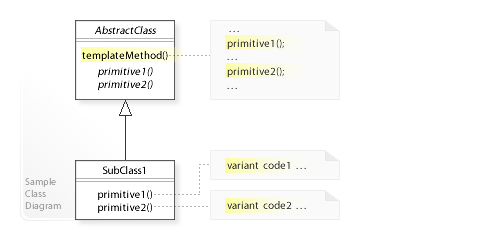
\includegraphics[width=8cm]{res/W3sDesign_Template_Method_Design_Pattern_UML.jpg}
    \caption{Template Method Pattern}
\end{figure}

\begin{itemize}
	\item 定义算法骨架:在抽象类中实现一个模板方法,这个方法定义了算法的骨架。通常,模板方法是一个具体的方法,它给出了一个顶层逻辑的骨架,而逻辑的组成步骤在相同类中以抽象操作的形式声明。
	\item 实现具体步骤:每一个抽象操作都由子类实现。这些操作通常被称为“钩子”或者“步骤”,子类将重写这些方法来提供具体的行为。
\end{itemize}

\subsection{模板方法应用举例}
\begin{lstlisting}[language=Java, caption=Template Method Design Pattern Example, label=lst:template_method_pattern]
public abstract class BulkItem {
	...
	public String getDescription() {
		return getSpecifics() + " in bulk";
	}
	protected abstract String getSpecifics();
	...
}

public class RainbowSweetFizzies extends BulkItem {
	protected String getSpecifics() {
		return "Rainbow Sweet Fizzies";
	}
}
\end{lstlisting}

假设有一个数据挖掘应用,它可以分析不同类型的数据集,比如 CSV 文件和 XML 文件。虽然每种数据格式的解析和分析过程有所不同,但基本的步骤是相同的,比如打开文件、读取数据、解析数据、分析数据和生成报告。

在这里,你可以创建一个带有一个名为 “analyze” 的模板方法的抽象类。这个模板方法会按顺序调用打开文件、读取数据、解析数据、分析数据和生成报告这些步骤。然后,你可以为 CSV 和 XML 数据集分别创建两个子类,它们实现 “analyze” 方法中那些特定于数据格式的步骤。

\subsection{评价模板方法}
模板方法具有以下优势:
\begin{itemize}
	\item 代码重用:通过将通用的算法结构定义在基类中,子类可以重用这部分代码。
	\item 灵活性:子类可以提供针对特定需求的实现,而不会破坏算法的整体结构。
	\item 封装:子类只需关注它们需要重写的特定步骤,而不是整个算法。
\end{itemize}

模板方法模式主要关注如何在保持算法结构稳定的同时,提供足够的灵活性,以便子类可以重写或重新定义算法的某些步骤。这种模式特别适合于那些算法步骤大致相同,但某些步骤的具体实现可能因情况而异的场景。

\section{Memento 备忘录模式}

Memento(备忘录)模式是一种行为设计模式,它的主要目的是保存一个对象的某个时刻的状态,以便可以在以后的某个时刻恢复对象到这个状态。备忘录模式在不违反封装的前提下捕获并外部化对象的内部状态,这样该对象就可以在以后将其状态恢复到先前的状态。

这种模式通常用于实现如撤销、恢复操作这样的功能,在诸如文档编辑器、代码编辑器、数据库事务的日志等多种应用中非常有用。

备忘录模式涉及三个主要元素:

\textbf{发起人(Originator):}
发起人是创建备忘录的对象,也是将来会使用备忘录来恢复其内部状态的对象。
它定义了创建备忘录和恢复自身状态的方法。

\textbf{备忘录(Memento):}
备忘录是一个用于存储发起人状态的对象。这个状态是根据发起人提供的信息来创建的。
备忘录防止发起人以外的其他对象访问备忘录。备忘录实际上有两个接口,一个是提供给负责人的宽接口,一个是提供给发起人的窄接口。

\textbf{负责人(Caretaker):}
负责人负责保存备忘录,但从不修改或查看其内容。
它保持备忘录的列表,提供了添加和检索备忘录的机制,允许对象在不同的时间点存储其状态,并在需要时恢复。

\subsubsection{工作流程}
\begin{itemize}
	\item 发起人根据其当前内部状态创建一个备忘录对象。
	\item 负责人获取并保存该备忘录。
	\item 当需要回滚到之前的状态时,负责人将这个备忘录返回给发起人。
	\item 发起人使用这个备忘录来恢复其内部状态。
\end{itemize}

\subsubsection{备忘录模式的优点}
\begin{itemize}
	\item 可以在不暴露对象实现细节的情况下保存和恢复对象的状态。
	\item 可以简化发起人的实现,因为它可以把负责管理状态历史的责任委托给负责人。
	\item 保留了对象的封装边界,简化了对象的接口。
\end{itemize}

\subsubsection{备忘录模式的缺点}
\begin{itemize}
	\item 如果发起人对象的内部状态大且复杂,频繁创建备忘录会消耗大量的系统资源。
	\item 负责人需要追踪发起人的历史记录,如果未经正确管理,这可能导致资源的过度使用。
\end{itemize}

在使用备忘录模式时,开发者需要平衡资源使用和系统设计的简洁性,并根据具体的应用场景和要求来决定是否使用这个模式。

\section{Visitor 访问者模式}
Visitor(访问者)模式是一种将算法与对象结构分离的软件设计模式。这种模式的基本想法是,它允许一个或多个操作应用于一组对象,而不改变这些对象的类。这里的“操作”可以是任何目的的过程,例如渲染到一个设备、序列化成多种格式等。通过使用访问者模式,可以在不修改现有类结构的情况下扩展功能。

访问者模式主要涉及以下几个组成部分:

\textbf{访问者(Visitor):}
这是一个接口或抽象类,用来声明访问操作,为每种具体的元素类(Element)声明一个访问操作。

\textbf{具体访问者(ConcreteVisitor):}
实现访问者声明的接口,每个操作实现算法的一部分,而该算法片段是对应于结构中对象的类。

\textbf{元素(Element):}
一个接口或抽象类,定义一个accept操作,它以一个访问者作为参数。

\textbf{具体元素(ConcreteElement):}
实现元素接口或继承自元素抽象类,实现accept方法,通常是visitor.visit(this)这样的形式。

\textbf{对象结构(ObjectStructure):}
可以是一个组合结构,或是一个集合,它知道如何枚举它的元素。
可能提供一个高层的接口以允许访问者访问它的元素。

\subsubsection{访问者模式的基本流程}

\begin{itemize}
	\item 客户端将具体访问者对象传递给对象结构。
	\item 对象结构接收到访问者后,它将这个访问者传递给它内部的每一个元素。
	\item 当元素接收到访问者,它们会调用访问者的方法,并将自身作为参数传递进去,从而使得访问者可以访问元素的具体类型。
\end{itemize}

\subsubsection{访问者模式的优点}

\begin{itemize}
	\item 符合单一职责原则,将数据操作和数据结构分离。
	\item 增加新的操作很容易,符合开闭原则,因为这只需要增加一个新的访问者类,而不需要修改现有的代码。
	\item 将具体元素类的状态和行为分离,状态作为参数传递给访问者,访问者用这些状态执行特定的行为。
\end{itemize}

\subsubsection{访问者模式的缺点}

\begin{itemize}
	\item 增加新的元素类比较困难,因为这需要在所有的访问者中增加新的方法。
	\item 破坏封装,因为访问者需要访问元素的内部状态。
	\item 可能会变得复杂,尤其是如果有很多不同的访问者或元素类。
\end{itemize}

在考虑使用访问者模式时,你应该考虑系统是否需要对对象结构中的元素执行多种不同且不相关的操作,并且不想让这些操作“污染”这些元素的类。如果是这样,访问者模式可能是一个很好的选择。

\section{Strategy 策略模式}

Strategy(策略)模式是一种行为设计模式,它定义了一系列算法,并将每一个算法封装起来,并使它们可以相互替换。策略模式让算法独立于使用它的客户端。这种类型的设计模式属于行为型模式。

策略模式适用于:
当你有多个类,它们之间的唯一区别是它们的行为时,可以使用策略模式,将这些行为封装成独立的策略类以实现不同的方式;当你需要在运行时切换算法时;当你的类包含多个条件语句,且这些条件依赖于该类的不同行为时。

它主要包含以下几个部分:

\textbf{上下文(Context):}
上下文通常会维护一个对策略对象的引用,它可以定义接口来让策略访问它的数据。
上下文接收客户端请求,并将请求委托给策略对象进行处理。

\textbf{策略(Strategy):}
是一个定义所有支持算法的公共接口。上下文使用这个接口来调用某个具体策略定义的算法。

\textbf{具体策略(ConcreteStrategy):}
实现策略接口,处理上下文请求。
具体策略包含了具体的算法或行为,它们是策略接口的具体实现。

\subsubsection{工作流程}

\begin{itemize}
	\item 客户端创建特定策略对象并传递给上下文。
	\item 上下文对象维护一个对策略对象的引用,用于执行其算法。
	\item 客户端可以通过修改上下文的策略对象来改变算法或策略。
\end{itemize}

\subsubsection{策略模式的优点}

\begin{itemize}
	\item 定义了一系列可重用的算法或行为。
	\item 避免使用多个条件语句(如 if...else 或 switch)。
	\item 可以提高算法的复用性和系统的可维护性。
	\item 客户端和策略算法解耦,简化了单元测试,因为每个算法都有自己的类,可以通过自己的接口单独测试。
\end{itemize}

\subsubsection{策略模式的缺点}

\begin{itemize}
	\item 客户端必须知道所有的策略类,并自行决定使用哪一个策略类。
	\item 策略模式会增加很多策略类或策略对象,但实际上这也体现了策略模式的可扩展性。
\end{itemize}

总的来说,策略模式是一种非常实用的模式,尤其是在你需要灵活地切换算法或行为的场景下。通过使用策略模式,你可以在运行时改变算法,增强代码的可维护性和可扩展性,并减少条件语句的复杂性。

\section{设计模式的集大成者---MVC设计模式}

创建用户界面 (User Interface, UI) 是计算机科学和软件工程中的一个复杂而关键的领域。以下是关于用户界面的关键概念和要点:

\textbf{系统状态的反映:}
用户界面的一个核心功能是展示系统的底层状态。无论是操作系统、应用程序还是网页,UI都是用户与系统交互的桥梁,反映了系统的当前状态。

\textbf{动态响应:}
当系统的状态发生变化时,用户界面必须相应地更新,以反映这些变化。例如,当一个文档被编辑或保存时,UI可能会更新其标题或状态图标。

\textbf{组件的层次性:}
UI通常由多个元素或组件组成。有些组件在功能上可能与整体UI相似,如大小调整功能。这种层次结构意味着UI设计必须考虑到每个组件如何独立和协同工作。

\textbf{关联性元素:}
有些界面元素总是与其他特定元素关联,并以某种方式修改或影响该元素。例如,滚动条允许用户在内容区域内滚动,并直接影响内容的查看方式。

\textbf{交互性:}
UI的另一个核心功能是为用户提供与系统互动的手段。这可能是通过按钮、菜单、滑块等UI元素来实现的。

\textbf{多种交互方式:}
用户可能有多种方式来执行特定的操作,例如,可以通过点击菜单项或使用键盘快捷键来执行命令。设计时要考虑这些不同的交互方式,并确保它们都能有效地工作。

\textbf{元素特定的行为:}
不同的UI元素可能有与之关联的不同的行为或操作。例如,一个播放按钮可能启动视频,而一个删除按钮可能删除列表中的项。

\textbf{系统功能的独立性:}
尽管UI是系统的前端和用户的交互点,但UI的设计和功能通常与系统的底层功能是分离的。这意味着可以在不改变底层系统的情况下更新或修改UI。

我们使用设计模式来解释用户界面的各个部分:

\textbf{系统状态的观察者:}
用户界面需要展示系统的底层状态。这里引入了观察者模式。观察者模式是一种设计模式,其中一个对象(被观察的对象)维护一个依赖于其状态的对象列表,并在其状态发生更改时通知它们。在这种情况下,用户界面是系统状态的观察者。

\textbf{组合和元素:}
用户界面由多个元素组成,有些元素的行为必须与整体用户界面相同,如大小调整。这里涉及到组合模式,其中对象组成树形结构,以表示部分-整体的层次关系。在用户界面中,这意味着单个元素和元素组(如面板或窗口)可以以相同的方式被视为和处理。

\textbf{装饰器模式:}
有些界面元素,如滚动条,总是与其他特定元素关联,并以某种方式修改或增强该元素的功能。装饰器模式允许在运行时动态地添加职责或行为到单个对象上。

\textbf{策略模式:}
用户界面为用户提供与其互动的手段,且具体如何执行特定操作可能会有所不同,如通过菜单或键盘快捷键。策略模式定义了一组算法,并将每个算法封装起来,使它们可以相互替换。这使得用户界面可以根据不同的上下文或用户偏好提供不同的交互策略。

\textbf{工厂方法模式:}
用户界面的不同元素可能有不同的关联操作。工厂方法模式提供了一个接口,用于创建对象,但允许子类决定实例化哪个类。在用户界面的上下文中,这可以用来定义和创建特定于元素的操作或行为。

\subsection{MVC模式}

MVC 是一种常用于开发用户界面的设计模式。它将应用程序逻辑分为三个主要组件:Model、View 和 Controller,以增加模块性和灵活性。MVC 是一个“原始”设计模式,存在于1980年之前,但其现代实现通常涉及其他设计模式的使用。就像其他设计模式一样,MVC 也有许多实现变体,以满足不同的需求和上下文。

\textbf{Model: }代表系统的状态或底层数据。当用户或 Controller 对 Model 进行更改时,它可能会通知其关联的 Views 进行更新。

\textbf{View: }展示 Model 的某种表示形式,通常是用户可见的界面部分。

\textbf{Controller: }作为 Model 和 View 之间的中介,控制用户的输入并更新 Model。

\subsubsection{与其他设计模式的关系}

\textbf{Observer: }当 Model 发生变化时,View 作为 Observer 会被通知并进行更新。这确保了 Model 的当前状态始终与用户界面同步。

\textbf{Composite: }用户界面经常有多个元素,其中某些元素(如面板或窗口)包含其他元素。Composite 模式允许我们将对象组合成树形结构,以表示部分-整体的层次关系。

\textbf{Decorator: }用于动态地给某个对象增加额外的职责,例如在 View 中增加滚动条或其他界面功能。

\textbf{Factory Method: }Controller 可能使用 Factory Method 来创建或实例化特定的对象或行为,根据需要进行操作。

\textbf{Strategy: }允许在运行时选择算法或操作的实现。在 MVC 中,Controller 可能使用不同的策略来处理不同的用户输入或操作。

\subsection{与用户界面有关的更改案例}

\subsubsection{Change what state of the system has to be shown}
这一点关注于系统中哪些状态需要展示给用户。这可能涉及到决策哪些数据或信息是关键的,哪些应该是可见的,以及哪些可能是次要的或应该被隐藏的。
更改要展示的系统状态可能是由于业务需求变化、用户反馈、或系统的功能更新。
这种变化可能会影响数据存储、数据处理和用户界面展示的方式。

\subsubsection{Change how the state of system is shown}
这涉及到如何向用户展示系统的状态。这可以是关于数据的可视化、界面的布局、颜色、字体或任何其他的界面元素。
更改状态的展示方式可能是为了提高用户体验、遵循品牌指南、或者是为了适应特定的设备或屏幕尺寸。
这也可能与采纳新的设计趋势或技术有关,例如从静态的展示过渡到动态的、交互式的展示。

\subsubsection{Change how the user performs actions in the system}
这关注于用户与系统交互的方式。这可能涉及到更改用户界面的元素,如按钮、菜单、滑块等,或更改用户完成任务的步骤和流程。
更改用户执行操作的方式可能是为了简化流程、增加新的功能、或基于用户的反馈和行为分析来提高效率和满足性。
这也可能涉及到技术的更新,例如引入语音命令、手势控制或其他新的交互方式。

\subsection{MVC与可变性}

MVC模式被设计出来的目的之一就是为了提高系统的可扩展性和可维护性。通过将业务逻辑、用户界面和用户输入分离到不同的部分,它允许开发者在不对整个系统造成太大冲击的情况下对某个部分进行更改。
\textbf{这种分离确保了在添加新功能或进行修改时,只需要对少数类进行更改,而不是对整个应用程序代码进行大规模的重写。新功能往往是在新类中添加的,而不是通过改变现有类来实现的($C$ decreased})。

\subsubsection{用更改案例分析可变性}

\subsubsection{Change what state of the system has to be shown}
当系统需要显示的状态发生变化时,主要的更改通常发生在“模型”中,因为模型负责处理应用程序的主要业务逻辑和数据。
与此同时,只需更改或添加受影响的“视图”,因为视图负责显示模型的数据。通常不需要更改任何控制器,因为控制器主要处理用户输入。
\subsubsection{Change how the state of system is shown}
当需要更改系统状态的显示方式时,通常只需更改相关的“视图”。这是因为视图定义了如何将模型的数据展示给用户。
在这种情况下,通常不需要更改模型或控制器,因为这种更改主要关注的是用户界面的外观和表现,而不是数据或用户输入。
\subsubsection{Change how the user performs actions in the system}
当需要更改用户如何在系统中执行操作时,只需更改或添加相关的“控制器”。控制器决定了如何响应用户的输入。
这里的文字似乎有些重复,因为它提到了通常不需要更改任何控制器,但考虑到上下文,这可能意味着不需要更改其他与特定操作无关的控制器。


\section{案例学习:JUnit}

JUnit利用了多种设计模式来组织其架构和功能,这有助于提高代码的可维护性、可扩展性和灵活性。

Test:
这是JUnit的主要接口,任何想要执行的测试都要实现此接口。
它有一个方法:run(TestResult)。
Composite:Component:
这是组合模式的组件部分。组合模式允许将对象组成树形结构以表示部分-整体的层次结构。
TestCase:
TestCase是JUnit中的核心类,代表一个测试用例。
它有多个方法,如:run(TestResult), runTest(), setUp(), 和 tearDown()。
setUp()和tearDown()方法用于测试前的初始化和测试后的清理。
它使用了Command和Template Method设计模式。
Command:它代表一个执行操作的指令。
Template Method:它定义了一个算法的框架,允许子类在不改变算法结构的情况下重定义算法的某些步骤。
TestSuite:
代表一个测试套件,可以包含多个测试用例。
它有两个主要方法:run(TestResult) 和 addTest(Test)。
这个组件利用了Composite模式,因为一个TestSuite可以包含其他的TestSuites或TestCases。
Composite:
代表组合模式中的组合部分,它可以包含其他组件。
TestResult:
用于收集测试的结果。
它使用了Collecting Parameter模式,这是一种将信息收集到一个对象中的方式,而不是将其散布到多个地方。
Adapter (Class):
适配器模式允许不兼容的接口工作在一起。这里的适配器模式可能被用来适配不同的测试类或方法。
Composite: Leaf 和 Pluggable Selector:
这些可能是JUnit中的高级特性或用于特定情况的组件。

\begin{lstlisting}[language=Java, caption=JUnit Case Study Example, label=lst:junit_case_study]
public abstract class TestCase extends Assert implements Test {
	public void runBare() throws Throwable {
		Throwable exception = null;
		setUp() ;
		try {
			runTest ();
		} catch (Throwable running) {
			exception = running;
		} finally {
			try {
				tearDown ();
			} catch (Throwable tearingDown) {
				if (exception == null) exception = tearingDown;
			}
		}
		if (exception != null) throw exception;
}
...
protected void setUp() throws Exception

protected void tearDown() throws Exception

}
\end{lstlisting}

\section{总结}
设计模式通常不会单独出现,往往会有其他模式紧随其后。
大多数设计模式都支持可变性,允许在新的类中提供新的功能。类中提供新功能,并减少需要更改的现有类的数量。
































